\subsection{Стабилизаторы}

\subsubsection{Staff}

Почему недостаточно просто воткнут  стабилитрон?\\
Потому что коэффициент стабилизации стабилитрона зависит от сопротивления нагрузки, чем оно меньше, тем меньше коэффициент стабилизации. Для увеличения этого параметра, однако могут быть применены эмиттерные повторители. 

\begin{center}
	\begin{figure}[h!]
		\center{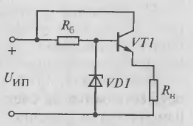
\includegraphics[scale=0.7]{stab_emrepiter.png}}
		\caption{Параметрический стабилизатор с эмиттерным повторителем}	
	\end{figure}
\end{center}

Но наличие эмиттерного повторителя привносит нестабильность в виде изменения непостоянства падения напряжения на эмиттерном переходе транзистора (температура и все такое). Ибо напряжение на выходе определяется следующим выражением:
\begin{equation}
U_n = U_{st} - U_{be}
\end{equation}

Поскольку изменение падания напряжения на выходе стабилизатора для больших сопротивлений нагрузки также зависит от изменения дифференциального сопротивления самого стабилитрона (который изменяется в общем случае нелинейно и зависит от проходящего тока), то имеет место следующее выражение (с линейной аппроксимацией, конечно):
\begin{equation}
\Delta U_{st} = \Delta I_{st} r_{st}
\end{equation}
Т.о. чтобы уменьшить колебания падения напряжения можно запитать стабилитрон с помощью генератора тока.
Соответствующая схема использует  транзистор, эмиттерный переход которого запитан с помощью стабилитрона, обеспечивающего РТ. 

\begin{center}
	\begin{figure}[h!]
		\center{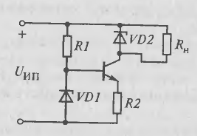
\includegraphics[scale=0.7]{GST_stab.png}}
		\caption{ГСТ подключенный к стабилитрону для получения опорного напряжение при большой $R_n$}	
	\end{figure}
\end{center}


Из закона Кирхгофа следует, что ток эмиттера равен 
\begin{equation}
I_e = \frac{U_{st1} - U_{be}}{R_2}
\end{equation}
Т.к. $B >>1 \Rightarrow (B+1) \approx B; U_{st1} >> U_{be} \Rightarrow I_k \approx I_e \approx \frac{U_{st1}}{R_2}$
Т.к. сопротивление нагрузки велико (необходимое допущение, ибо строим источник опорного напряжения), то весь ток коллектора проходит через стабилитрон VD2, следовательно $\Delta I_{st} r_{st} \longrightarrow 0$\\

Далее рассмотрим непрерывный (не импульсный) стабилизатор напряжения.\\

\begin{center}
	\begin{figure}[h!]
		\center{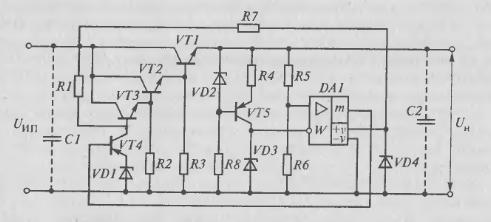
\includegraphics[scale=0.7]{stab_with_emp.png}}
		\caption{Схема стабилизатора с непрерывной стабилизацией.}	
	\end{figure}
\end{center}



Здесь функции источника опорного напряжения выполняют следующие компоненты:
VD2, VD3, VT5, R8, R4.\\
Опорное напряжение сравнивается с разделенным пропорционально резисторам R5 и R6. Разница данных сигналов усиливается дифференциальным усилителем DA1 (было бы замечательно поставить туда операционник, наверно, но в оригинале имеется ввиду именно дифференциальный усилитель).


Поскольку при нулевой разнице сигналов на входи диф. усилителя от все еще генерирует примерно половину напряжения питания (постоянное напряжение), то стабилитрон VD1 должен равняться этой половине(т.е. не пропускать ток при нулевой разнице) т.е. его напряжение стабилизации должно быть в 2 раза меньше чем напряжение стабилизации стабилитрона VD4.


\textbf{Импульсный стабилизатор.}


Суть заключается в том, чтобы манипулировать выходным напряжением открывая и закрывая ключ. Импульсы затем можно сгладить с помощью LC-фильтра.

\begin{center}
	\begin{figure}[h!]
		\center{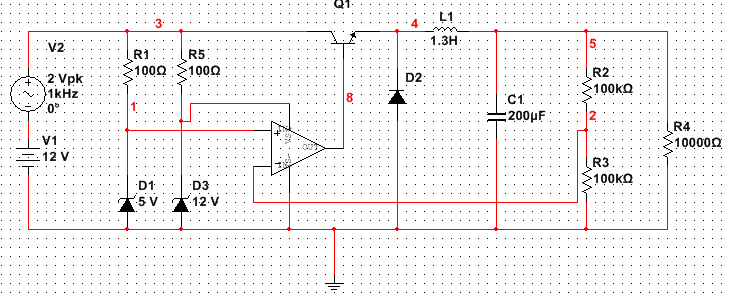
\includegraphics[scale=0.7]{impult_stab.png}}
		\caption{Простейший импульсный стабилизатор с понижающей схемой включения.}	
	\end{figure}
\end{center}

Здесь в качестве ключа используется транзистор в режиме насыщения  (полевой лучше). Операционный усилитель при напряжении, меньшем чем опорное, открывает транзистор, тем самым заряжая катушку/конденсатор. 


Опорное напряжение гарантируется стабильным т.к. входное сопротивление ОУ достаточно бесконечно для этого.
Но для большого улучшения можно использовать стабилитрон с ГСТ, как это делалось ранее.


Для предотвращения КЗ можно применить следующею self-made фичу:

\begin{center}
	\begin{figure}[h!]
		\center{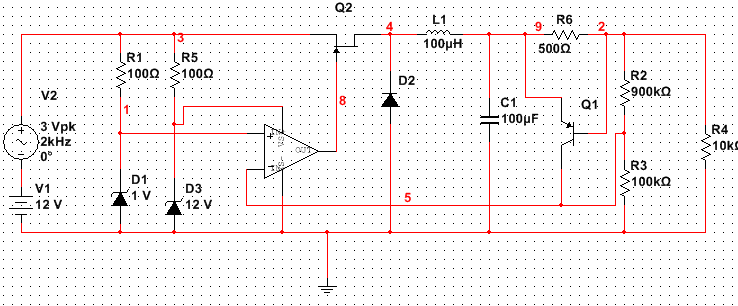
\includegraphics[scale=0.7]{imp_stab_KZ.png}}
		\caption{Защита от КЗ}	
	\end{figure}
\end{center}
Принцип ее можно применять и к стабилизаторам постоянного действия.
Суть такова, что при КЗ ток большой и на контрольном резисторе падает достаточно напряжение для того, чтоб открыть транзистор, который закроет подачу тока. Т.о. напряжение в цепи упадет до 1/10 в данном случае.

